\section{Desarollo packet pincer}

En esta sección veremos el funcionamiento de cada parte de la herramienta, la cual se ha llamado 'packet pincer' por el momento. Veremos qué y cuáles argumentos de consola acepta, como realiza la lectura de paquetes tanto en tiempo real como por trazas. A continuación se explicarán los diferentes pasos que llevan a cabo en el momento al analizar un paquete y como se realiza la generación de estadísticas. Finalmente, veremos como se realiza el etiquetado automático de los flujos y se escriben emiten los resultados.

El flujo principal de la aplicación se puede observar en la Figura \ref{fig:packetpincerexecution}. Como podemos ver, se van extrayendo paquetes mientras se encuentren disponibles. Cuando se obtiene uno, en caso de ser un paquete IPv4 fragmentado, se intenta reconstruir o se guarda en caso de no poder. A continuación, se comprueba si la herramienta soporta analizar el paquete indicado y, en caso afirmativo, acumula la información en el flujo de transporte respectivo. Finalmente, se 'cierran' los flujos antiguos, es decir, se emite la información relevante y a continuación se descarta el resto de información acumulada.

\begin{figure}[H]
  \begin{center}
    \centering
    \resizebox{!}{\dimexpr\textheight-2\baselineskip\relax}{%
      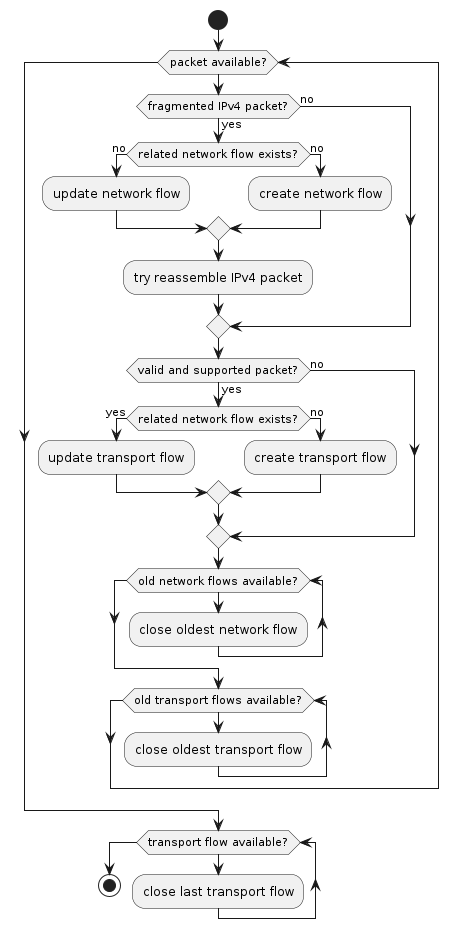
\includegraphics{plant_uml_diagrams/general_tool_loop.png}
    }
  \end{center}
  \caption{Flujo de la aplicación durante su ejecución}\label{fig:packetpincerexecution}
\end{figure}

\subsection{Argumentos y señales}

El programa está pensado para ser ejecutado desde el terminal. Debido a esto, hemos de definir que argumentos se pueden pasar al programa y hacer que este reaccione a señales del sistema operativo. Los argumentos suelen ser pasados desde el mismo comando utilizado para ejecutar el programa, siendo un ejemplo '\texttt{packet\_pincer \underline{help}}'. Las señales a su vez se pueden enviar utilizando una combinación de teclado como \texttt{CTRL+C} o utilizando otro programa.

Para hacer la gestión de los argumentos enviados por el terminal, se ha hecho uso de la librería (o 'crate', en la nomenclatura utilizada en Rust) clap \cite{Knapp_clap_2024}. Concretamente, se ha hecho uso de la funcionalidad 'derive', la cual permite expresar los argumentos a pasar como un tipo del lenguaje de forma declarativa. Adicionalmente, la librería añade diversas funcionalidades que mejoran la experiencia de usuario. A partir de nuestras definiciones, se muestran unas indicaciones de uso si se ejecuta \texttt{packet\_pincer --help} o si se pasan argumentos inválidos. Los argumentos definidos para el programa consisten en:

\begin{enumerate}
  \item Opcionalmente indicar si escribir los resultados generados en archivos (indicando su prefijo), en la salida estándar o no emitir nada.
  \item Opcionalmente indicar si un archivo en formato csv de las etiquetas que han de ponerse en los flujos. En caso de que se especifique este archivo y no haya etiqueta correspondiente, se generará una llamada 'benign'.
  \item Indicación del origen de los paquetes a analizar. Este puede ser 'offline' (a partir de una traza de red o un directorio de estas) u 'online' (a partir de una interficie de red).
\end{enumerate}

Respecto a las señales, se hace uso de la librería ctrlc \cite{controlc}. Esta permite detectar señales de interrupción enviadas por el usuario para interrumpir la ejecución de la aplicación. Si el programa no respondiese a estas señales, el sistema operativo terminaría el proceso directamente. Esto podría provocar la escritura parcial de los archivos, potencialmente corrompiéndolos. En caso de que se genere una señal de interrupción del programa, lo tratamos como que no hay más paquetes disponibles.

El código que se encarga de tratar estos puntos, se puede encontrar en \texttt{main.rs} en el anexo 2 o en el repositorio de GitHub.

\subsection{Lectura de paquetes en tiempo real}

Por hacer

\subsection{Lectura de trazas de paquetes}

Por hacer

\subsection{Extensión de libreria de código abierto para la decodificación de paquetes}

Por hacer

\subsection{Defragmentación IPv4}

Por hacer

\subsection{Separación de flujos}

Por hacer

\subsection{Generación de estadísticas}

Por hacer

\subsection{Escritura y etiquetado de flujos}

Por hacer

